\clearpage
\fancyhead[R]{\sffamily\small\color{Muted}Vulkan / 材质发光}
\section{火盆的自发光绘制}
Sun Temple 中央的火盆只占画面一小块。初版为了算出哪些炭火能被相机看见，又画了一遍房间里的全部网格。其实主绘制已经留下了离相机最近的表面深度。再画火盆时，只要它在某个像素的深度等于已存深度，这个像素就有机会发光；挡在前面的柱子已经决定了遮挡，无需重画。

\begin{figure}[H]\centering
\begin{minipage}[c]{.635\linewidth}\centering
\begin{tikzpicture}
\node[anchor=south west,inner sep=0] (photo) at (0,0) {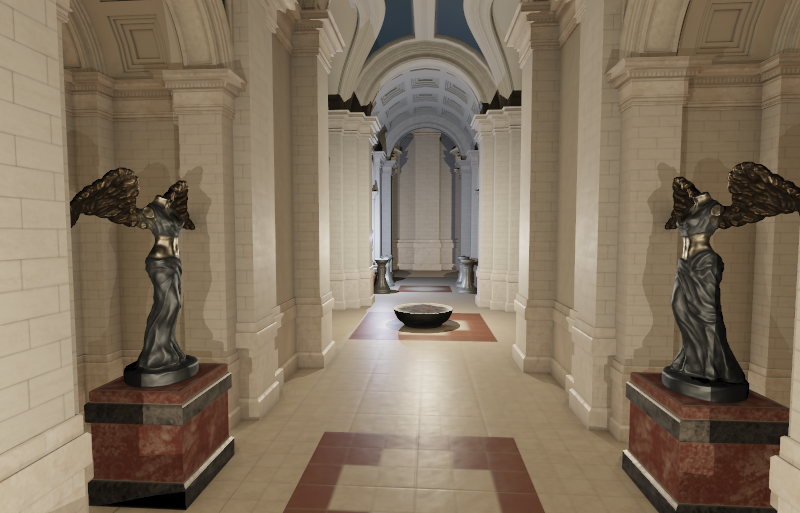
\includegraphics[width=\linewidth]{emissive-material/temple.png}};
\begin{scope}[x={(photo.south east)},y={(photo.north west)}]
\draw[white,line width=1.4pt] (.43125,.31774) rectangle (.59875,.54386);
\draw[Rust,line width=.65pt] (.43125,.31774) rectangle (.59875,.54386);
\end{scope}
\end{tikzpicture}
\end{minipage}\hfill
\begin{minipage}[c]{.32\linewidth}\centering
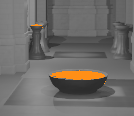
\includegraphics[width=\linewidth]{emissive-material/temple-emission.png}
\end{minipage}
\caption{左图是正式编辑器第 24 帧的面板颜色。右图放大方框，橙色标出回放中发光值大于零的 396 个像素，灰色保留火盆的轮廓。两版全部 410\,400 个像素的线性光照与显示颜色分别逐字节相同。}
\end{figure}

{\smalltable\noindent\begin{tabularx}{\linewidth}{@{}Xrr@{}}\toprule
同一帧的工作 & 重画全部网格 & 沿用主表面深度\\\midrule
发光绘制次数 & 48 & 4\\
这些绘制读取的索引数 & 1\,819\,128 & 202\,122\\
发光绘制的 GPU 时间（微秒） & 169.73 & 16.83\\
将发光加入场景的 GPU 时间（微秒） & 10.75 & 16.29\\\bottomrule
\end{tabularx}\par}

新版只提交四个发光网格。两片材质若恰好共面，光凭深度无法分出先后。主绘制把胜出的材质是否发光记在底色图里，合成时多读一次这个标记，因此表中最后一项稍慢。两版均保留 48 次主表面绘制、48 次拾取绘制与 22 次界面绘制。宽高为 $800\times513$ 时，发光图和合成结果合计 12.52\,MiB。沿用深度可少存一张 D32 图，省去 1.57\,MiB 像素数据；这里按格式计算，驱动分配对齐另计。

设备是 RTX 5070 Ti Laptop GPU，Debug x64，Vulkan 验证开启。每份 RenderDoc 1.47 捕获先回放一次，再测 11 次，表中为中位数。两版模型顶点因新增发光 UV 从 44 增至 52 字节。CPU 在这一次捕获中进入各条 \code{vkCmdDrawIndexed} 的耗时之和为 121 与 32 微秒，其中包括截帧开销。另用没有发光材质的古董相机复查，两个版本均为 29 次绘制、9 次计算，颜色逐像素相同。

{\small\color{Muted}原帧、逐次读数和复查命令见 \path{output/profiling/emissive-material/}。\par}
